\begin{frame}\frametitle {Real-$\gamma$ Background. Sources}

Main sources of true $\gamma$ background are $Z\gamma$ and $W\gamma \rightarrow \tau \nu \gamma$. The MC-based estimation is used to subtract these backgrounds.

MC-based background estimation.
  \begin{figure}[htb]
    \begin{center}
       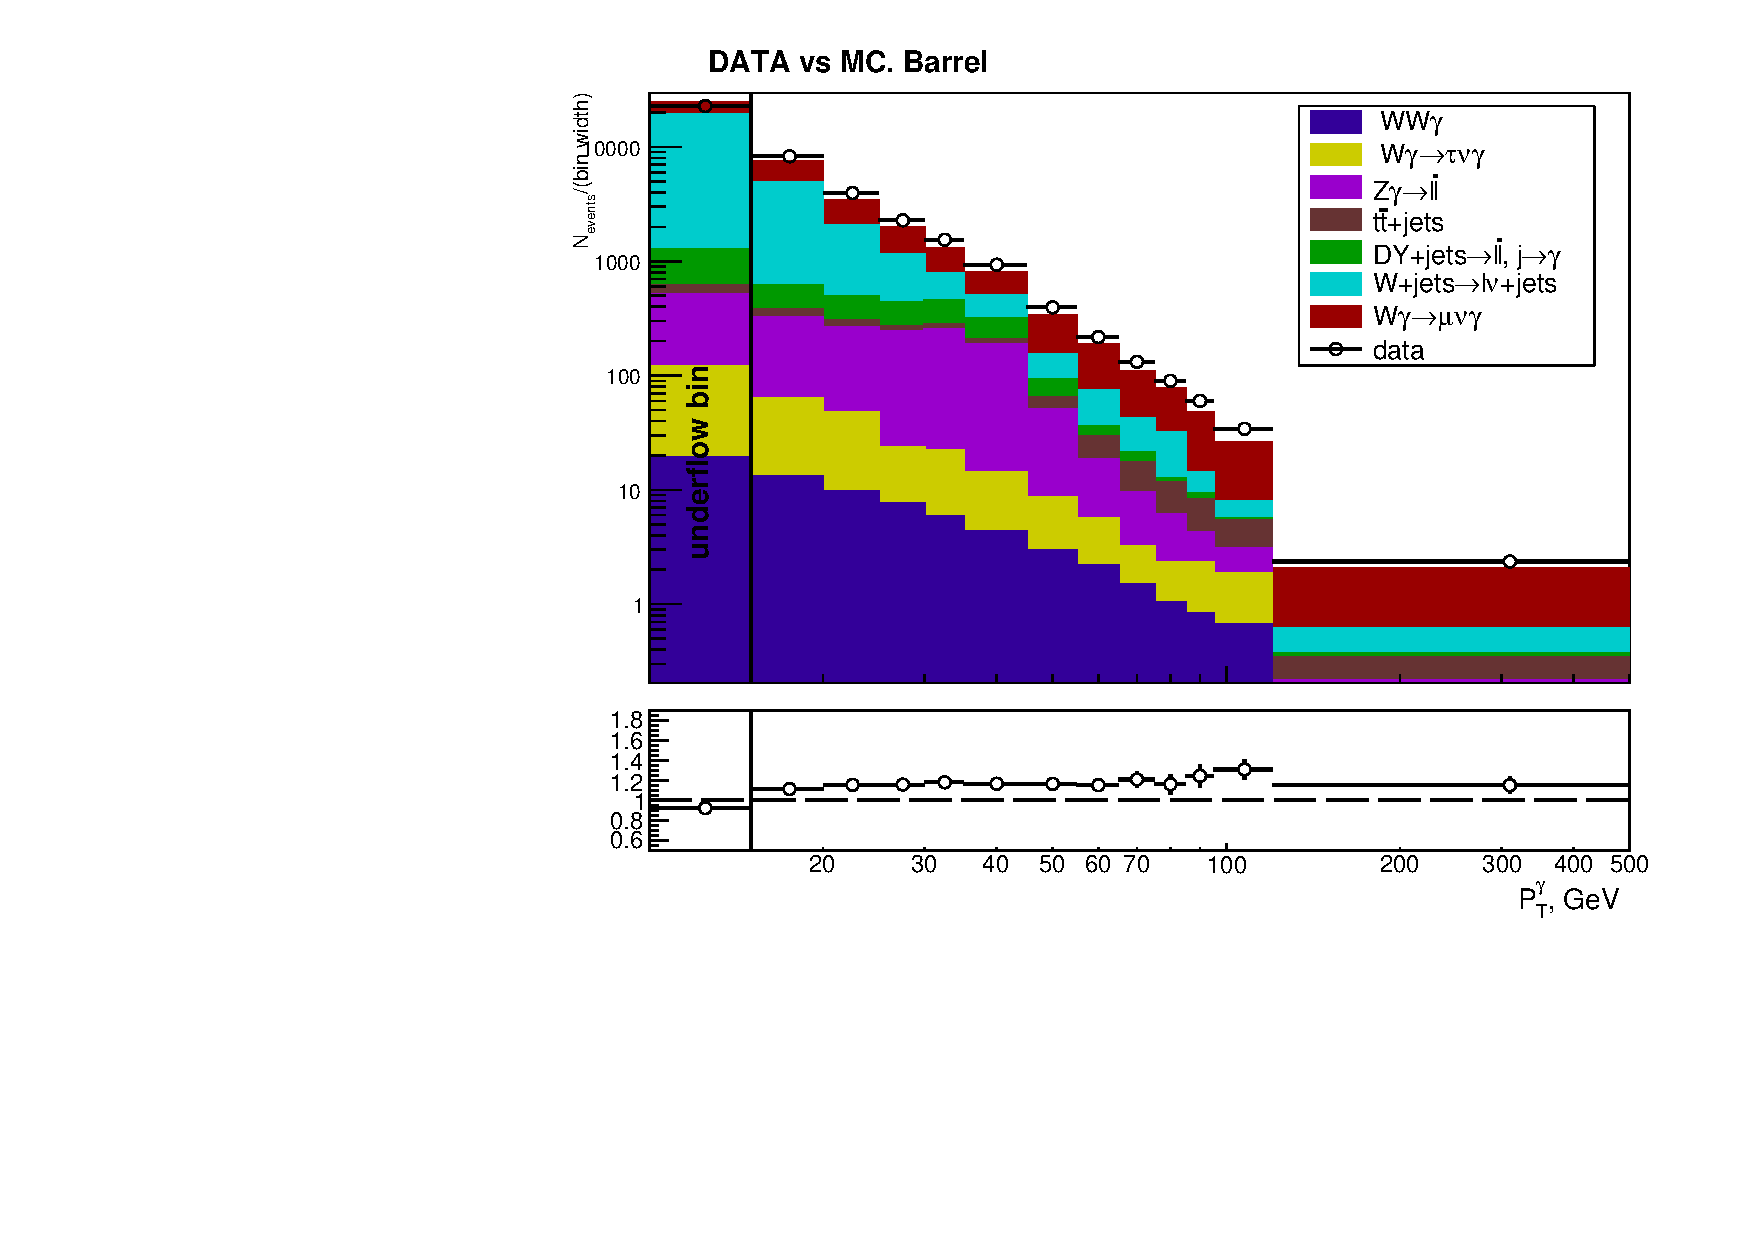
\includegraphics[width=0.40\textwidth]{../figs/figs_v11/MUON_WGamma/PrepareYields/c_TotalDATAvsMC_Barrel__phoEt.pdf}
    \end{center}
  \end{figure}
\end{frame}%{Real-$\gamma$ Backgrounds}

\begin{frame}\frametitle{\footnotesize{$P_T^{\gamma}$ Spectrum (EB only)}}
   \begin{figure}[htb]
    \begin{center}
       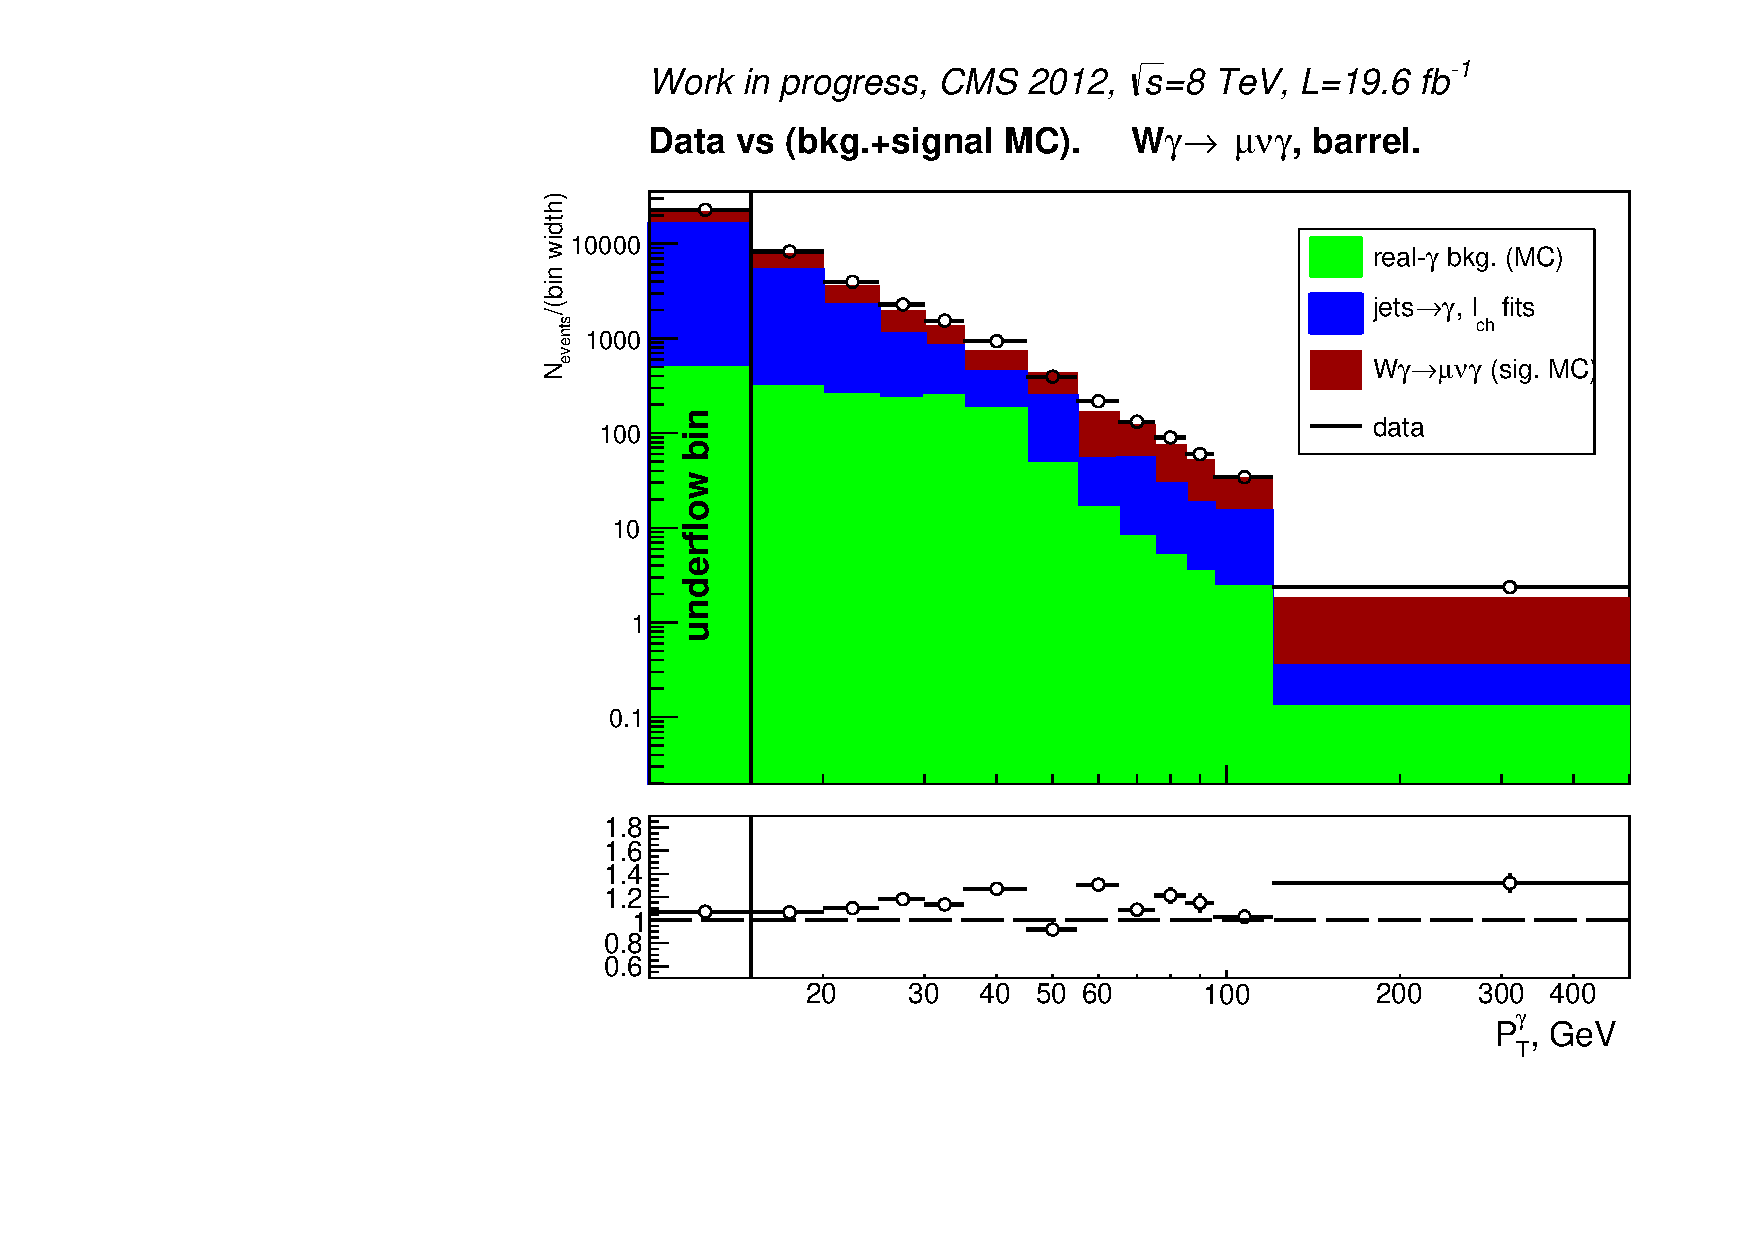
\includegraphics[width=0.40\textwidth]{../figs/figs_v11/MUON_WGamma/PrepareYields/c_DATAvsBkgPlusSigMCc_MUON_WGamma_TEMPL_CHISO_UNblind__Barrel__phoEt.pdf}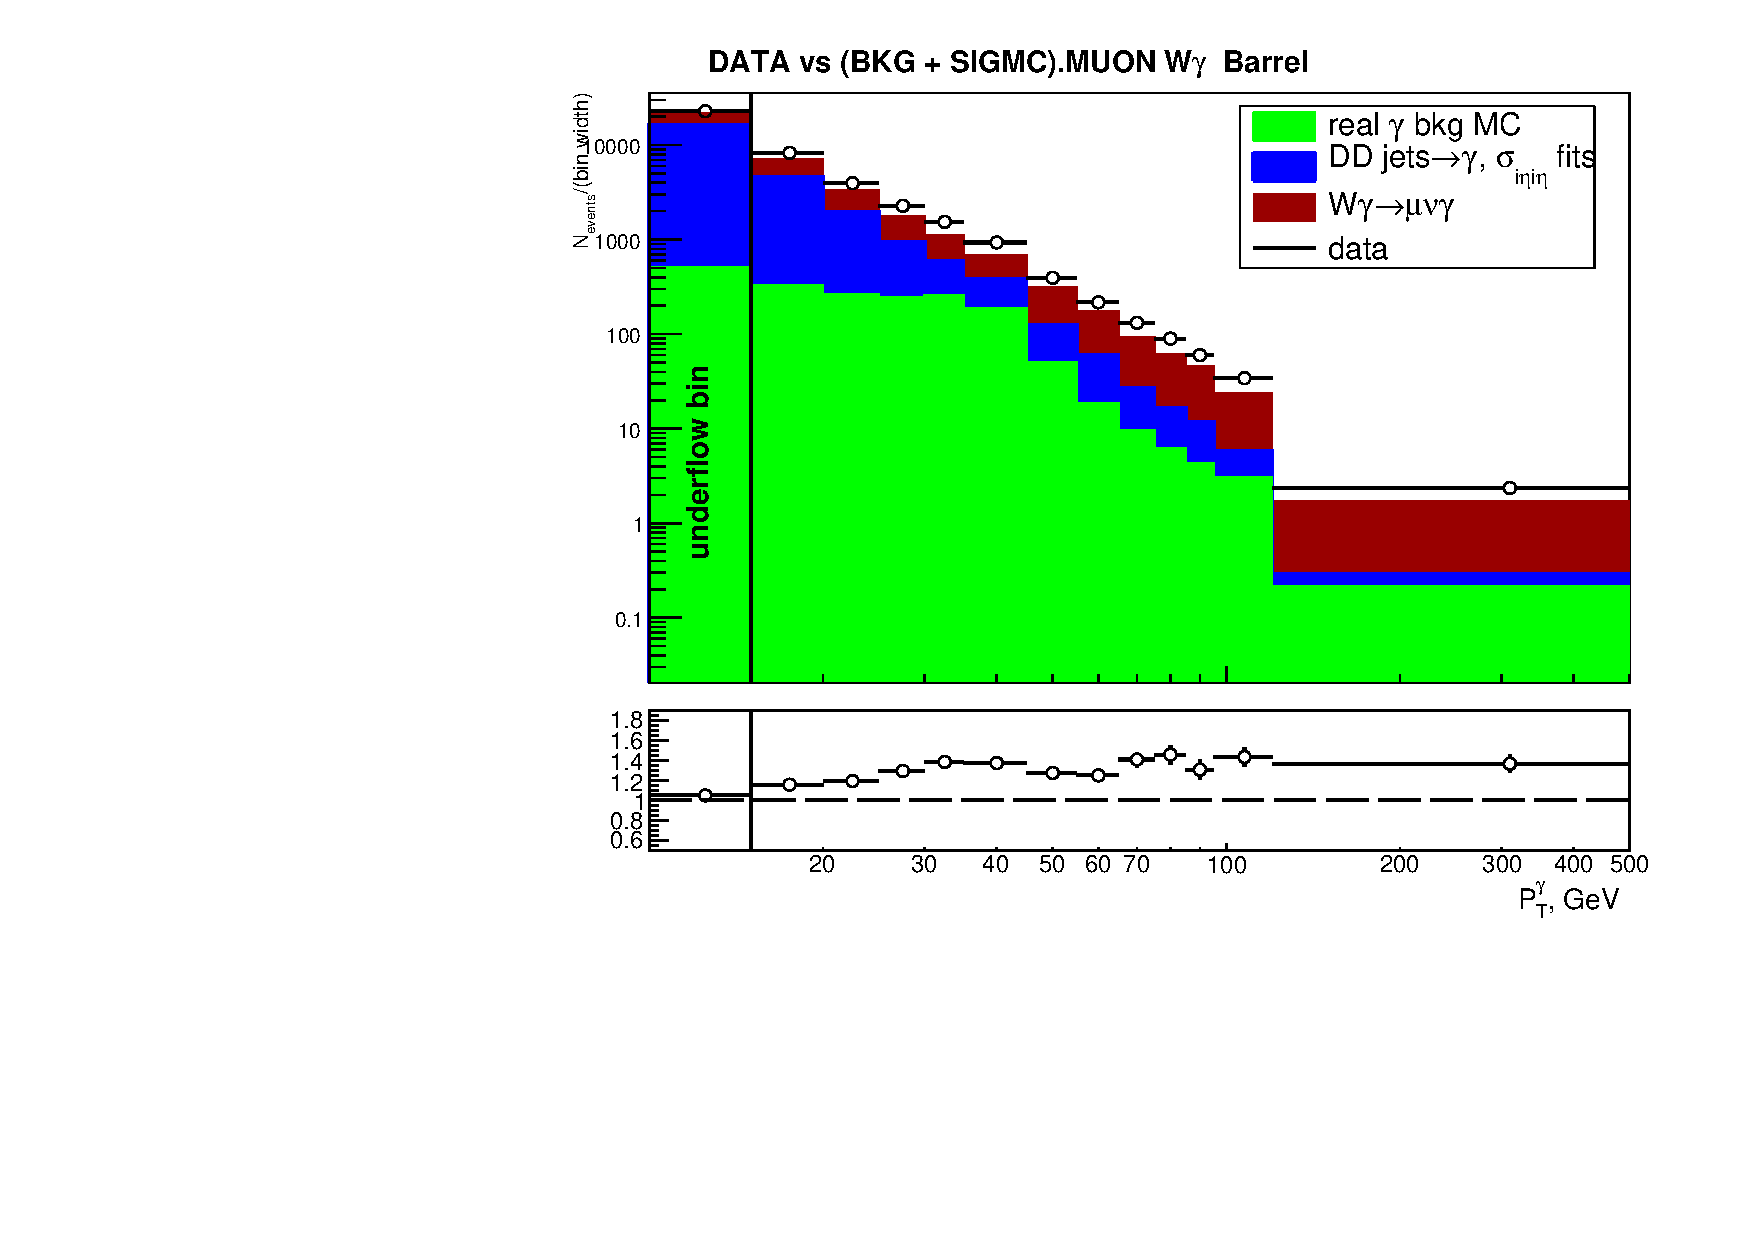
\includegraphics[width=0.40\textwidth]{../figs/figs_v11/MUON_WGamma/PrepareYields/c_DATAvsBkgPlusSigMCc_MUON_WGamma_TEMPL_SIHIH_UNblind__Barrel__phoEt.pdf}\\
       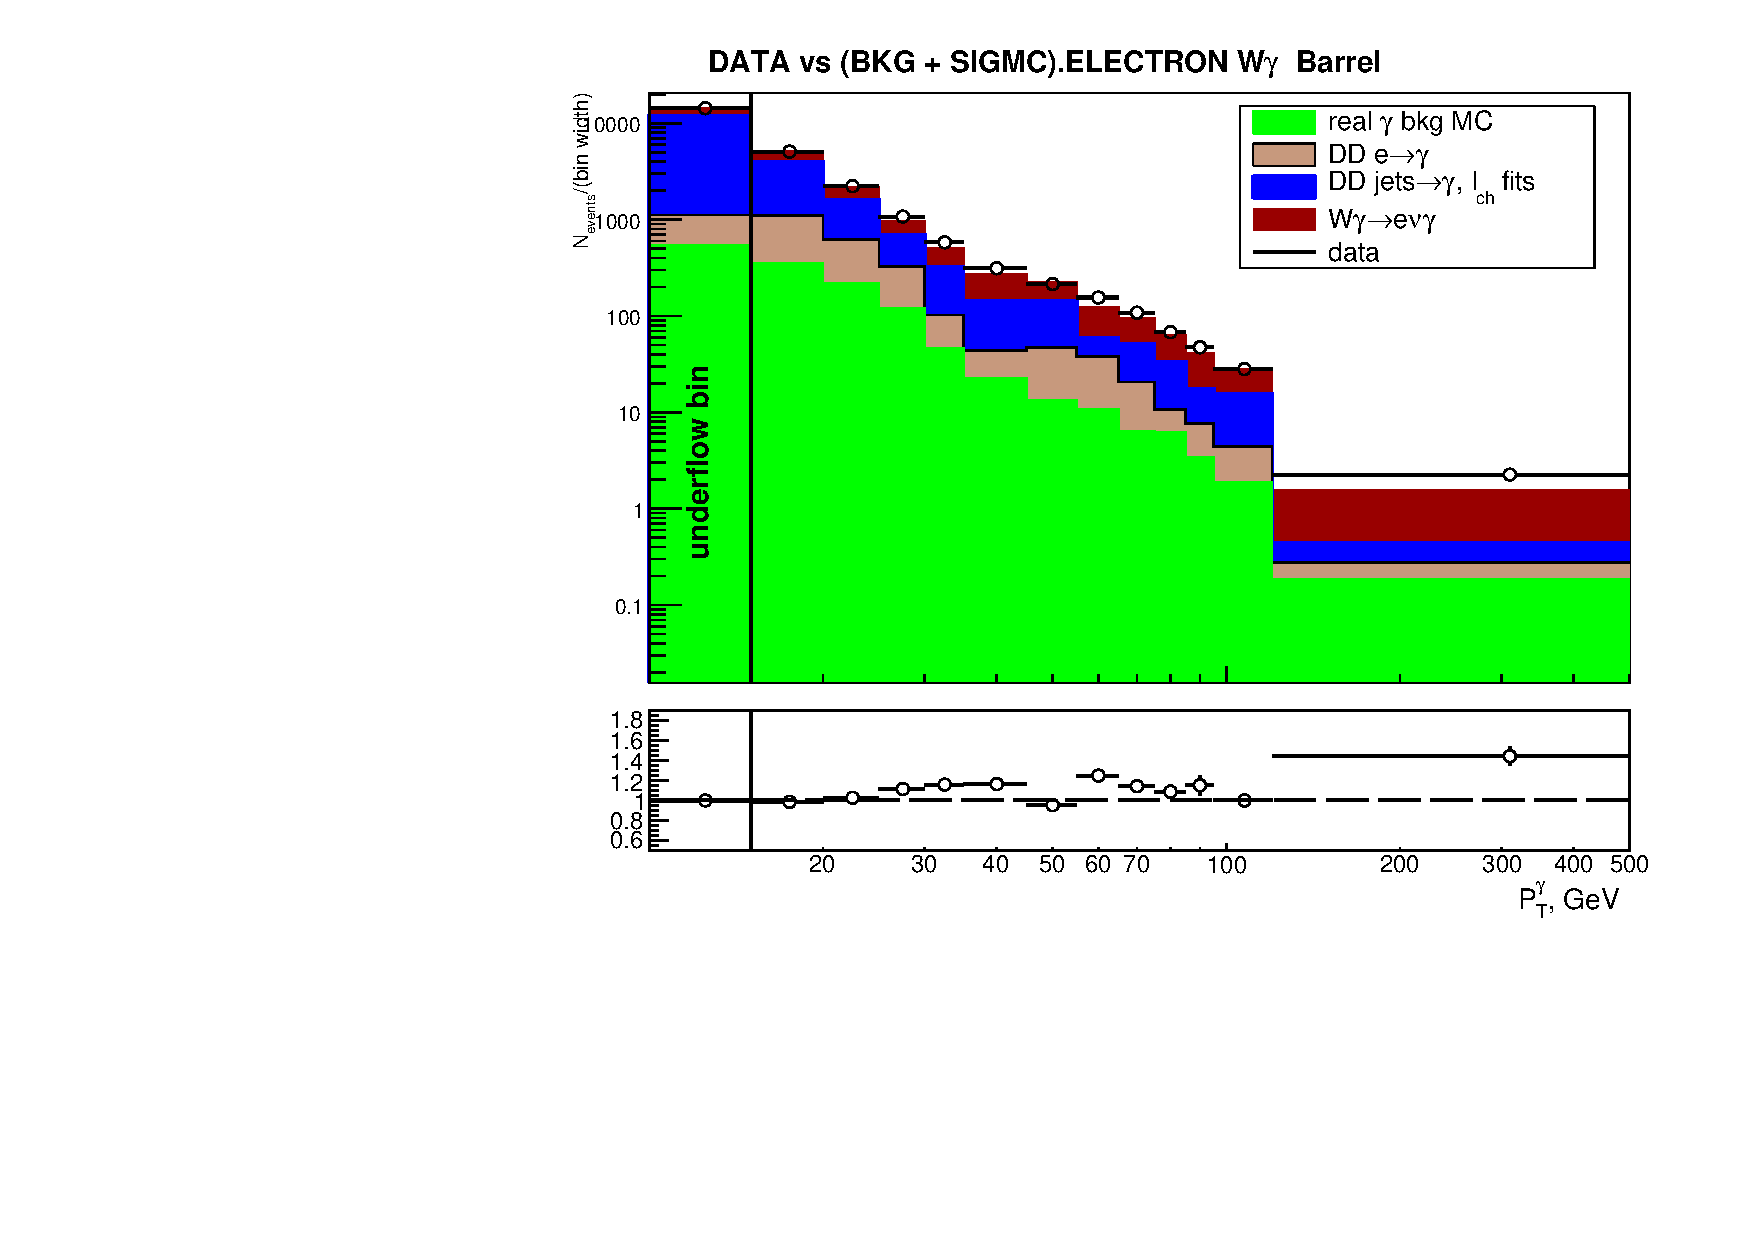
\includegraphics[width=0.40\textwidth]{../figs/figs_v11/ELECTRON_WGamma/PrepareYields/c_DATAvsBkgPlusSigMCc_ELECTRON_WGamma_TEMPL_CHISO_UNblind__Barrel__phoEt.pdf}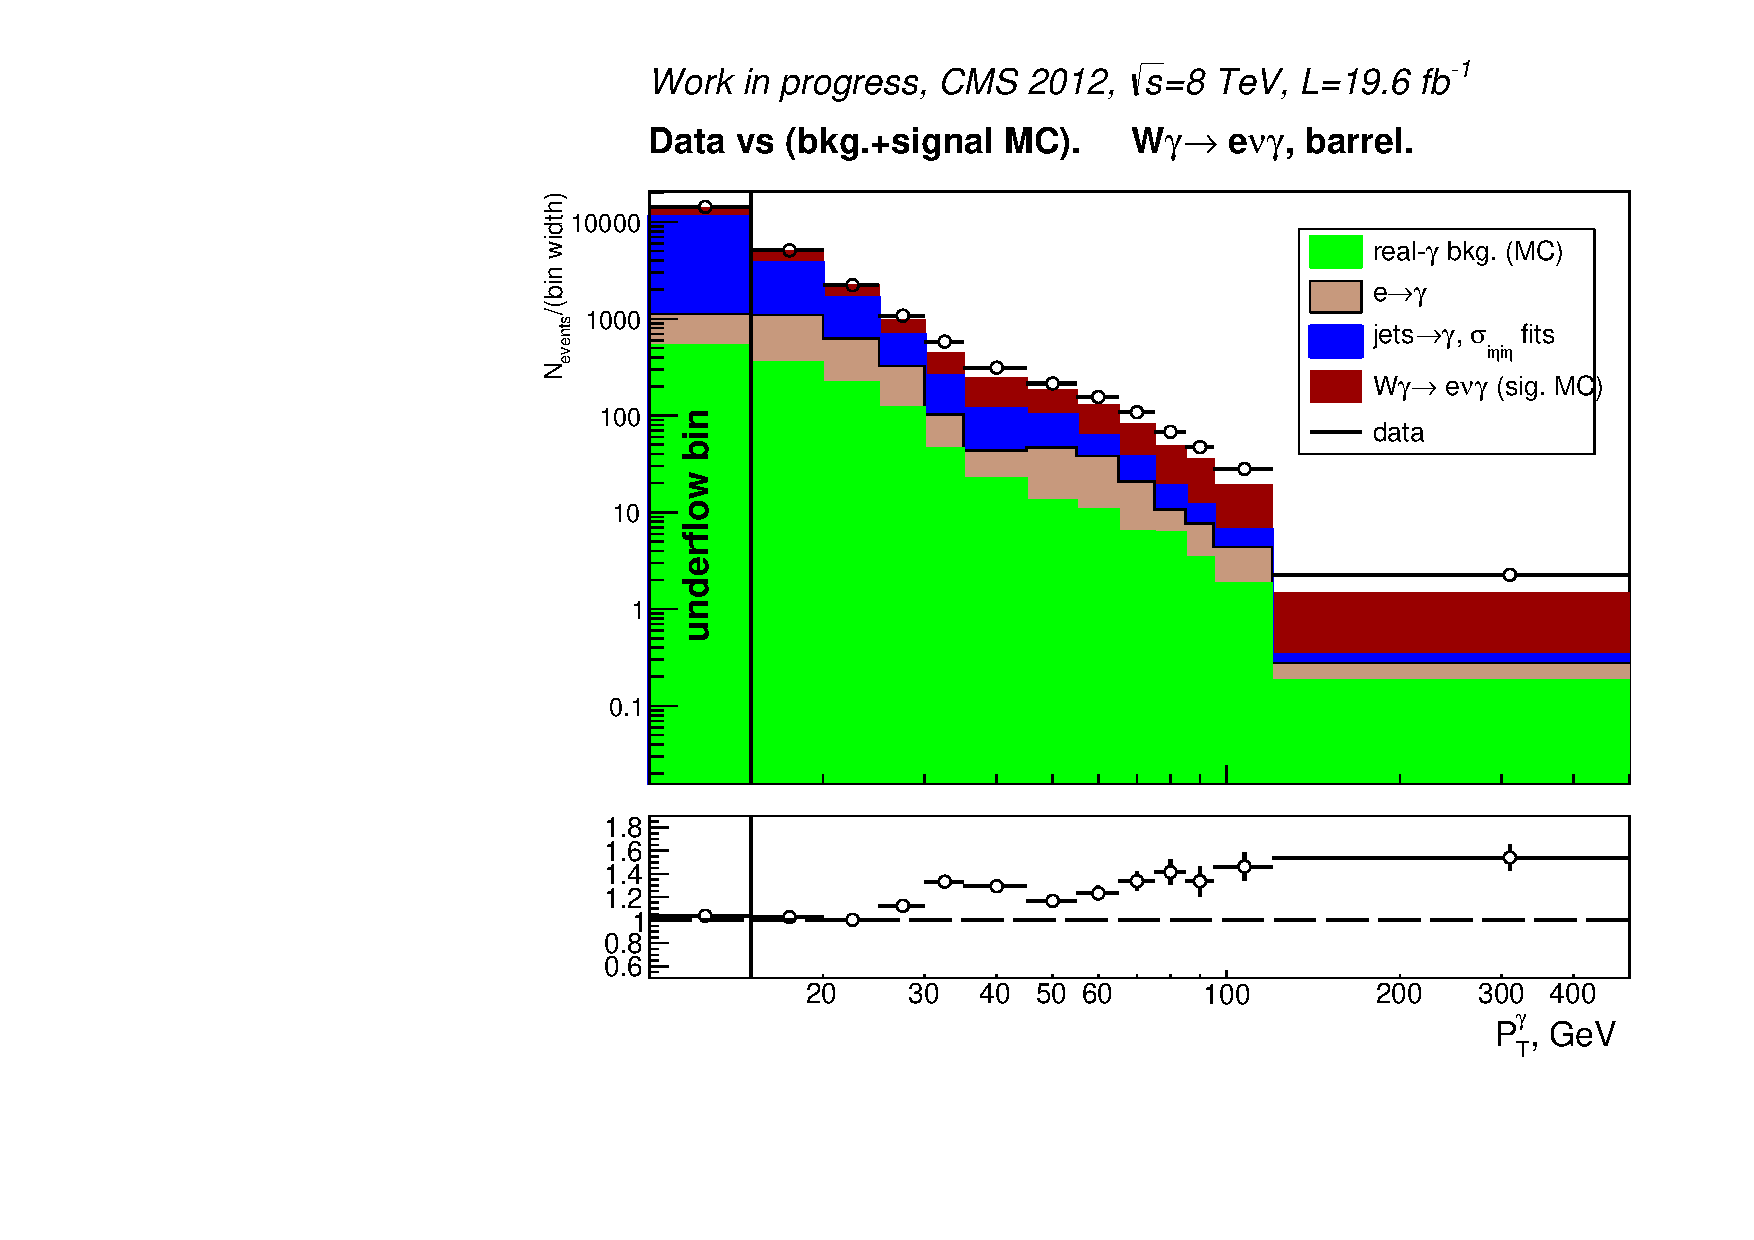
\includegraphics[width=0.40\textwidth]{../figs/figs_v11/ELECTRON_WGamma/PrepareYields/c_DATAvsBkgPlusSigMCc_ELECTRON_WGamma_TEMPL_SIHIH_UNblind__Barrel__phoEt.pdf}\\
    \end{center}
  \end{figure}
\end{frame}%{$jets \rightarrow \gamma$ Background Subtraction. Plots, W$\gamma$}

\begin{frame}\frametitle{\footnotesize{$P_T^{\gamma}$ Spectrum after Background Subtraction (EB and EE)}}
  
  \begin{figure}[htb]
    \begin{center}    
       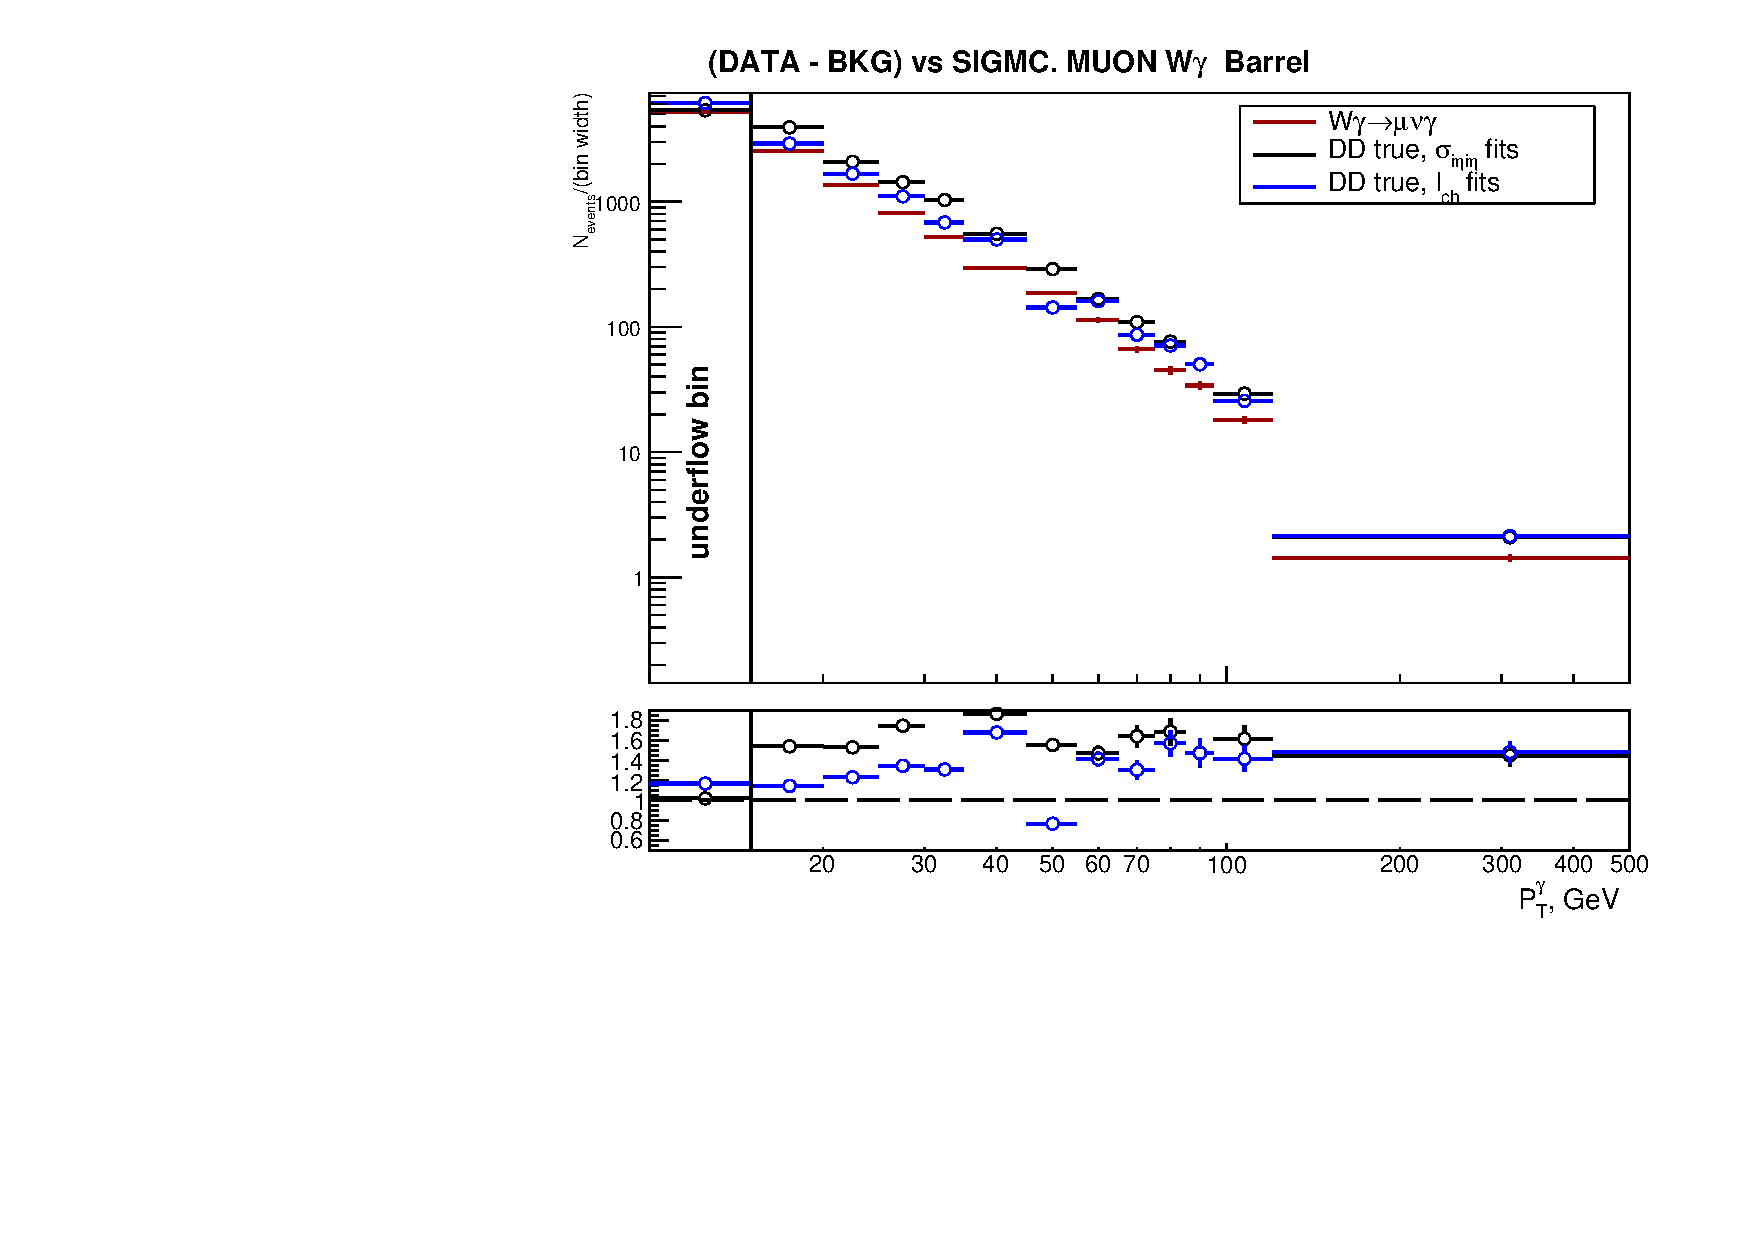
\includegraphics[width=0.40\textwidth]{../figs/figs_v11/MUON_WGamma/PrepareYields/c_BkgSubtrDATAvsSIGMC_c_MUON_WGamma__UNblind__Barrel__phoEt.pdf}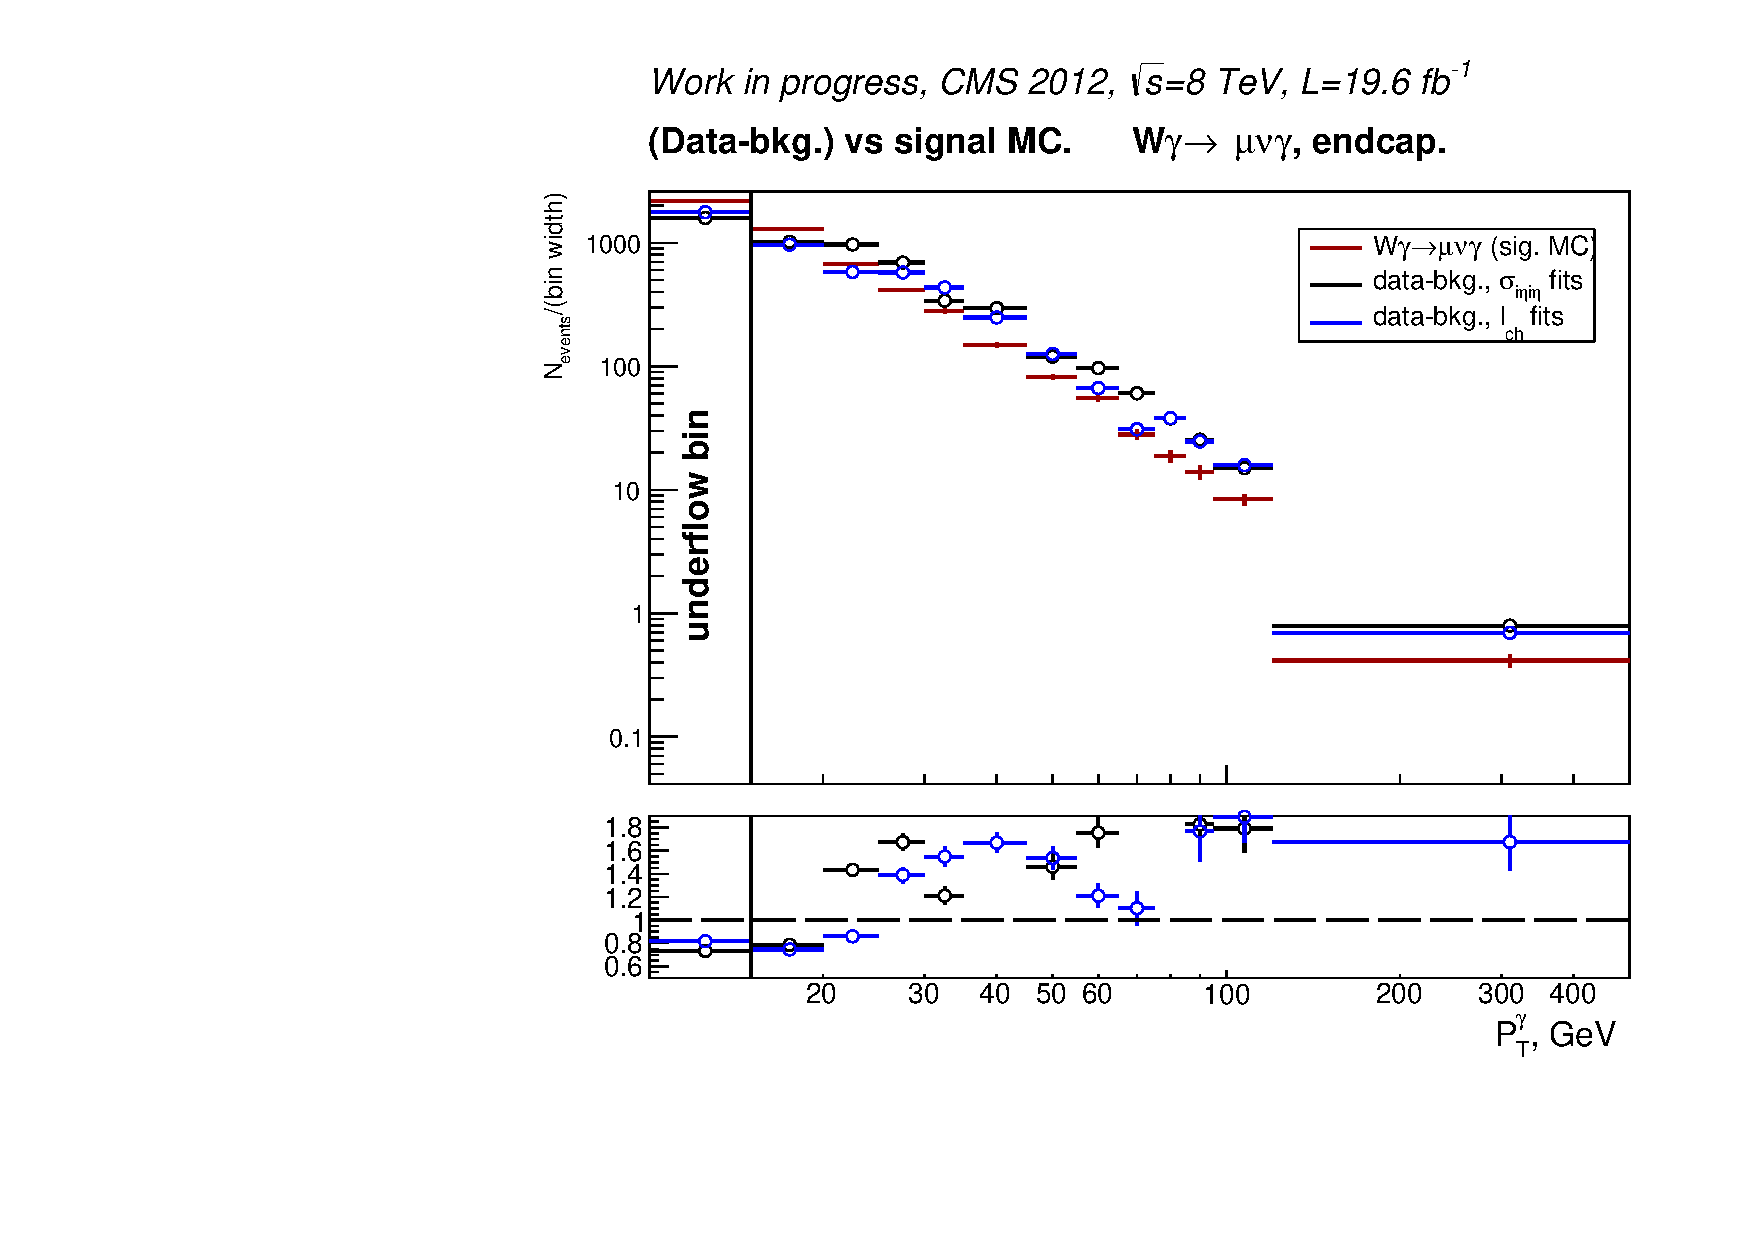
\includegraphics[width=0.40\textwidth]{../figs/figs_v11/MUON_WGamma/PrepareYields/c_BkgSubtrDATAvsSIGMC_c_MUON_WGamma__UNblind__Endcap__phoEt.pdf}\\
       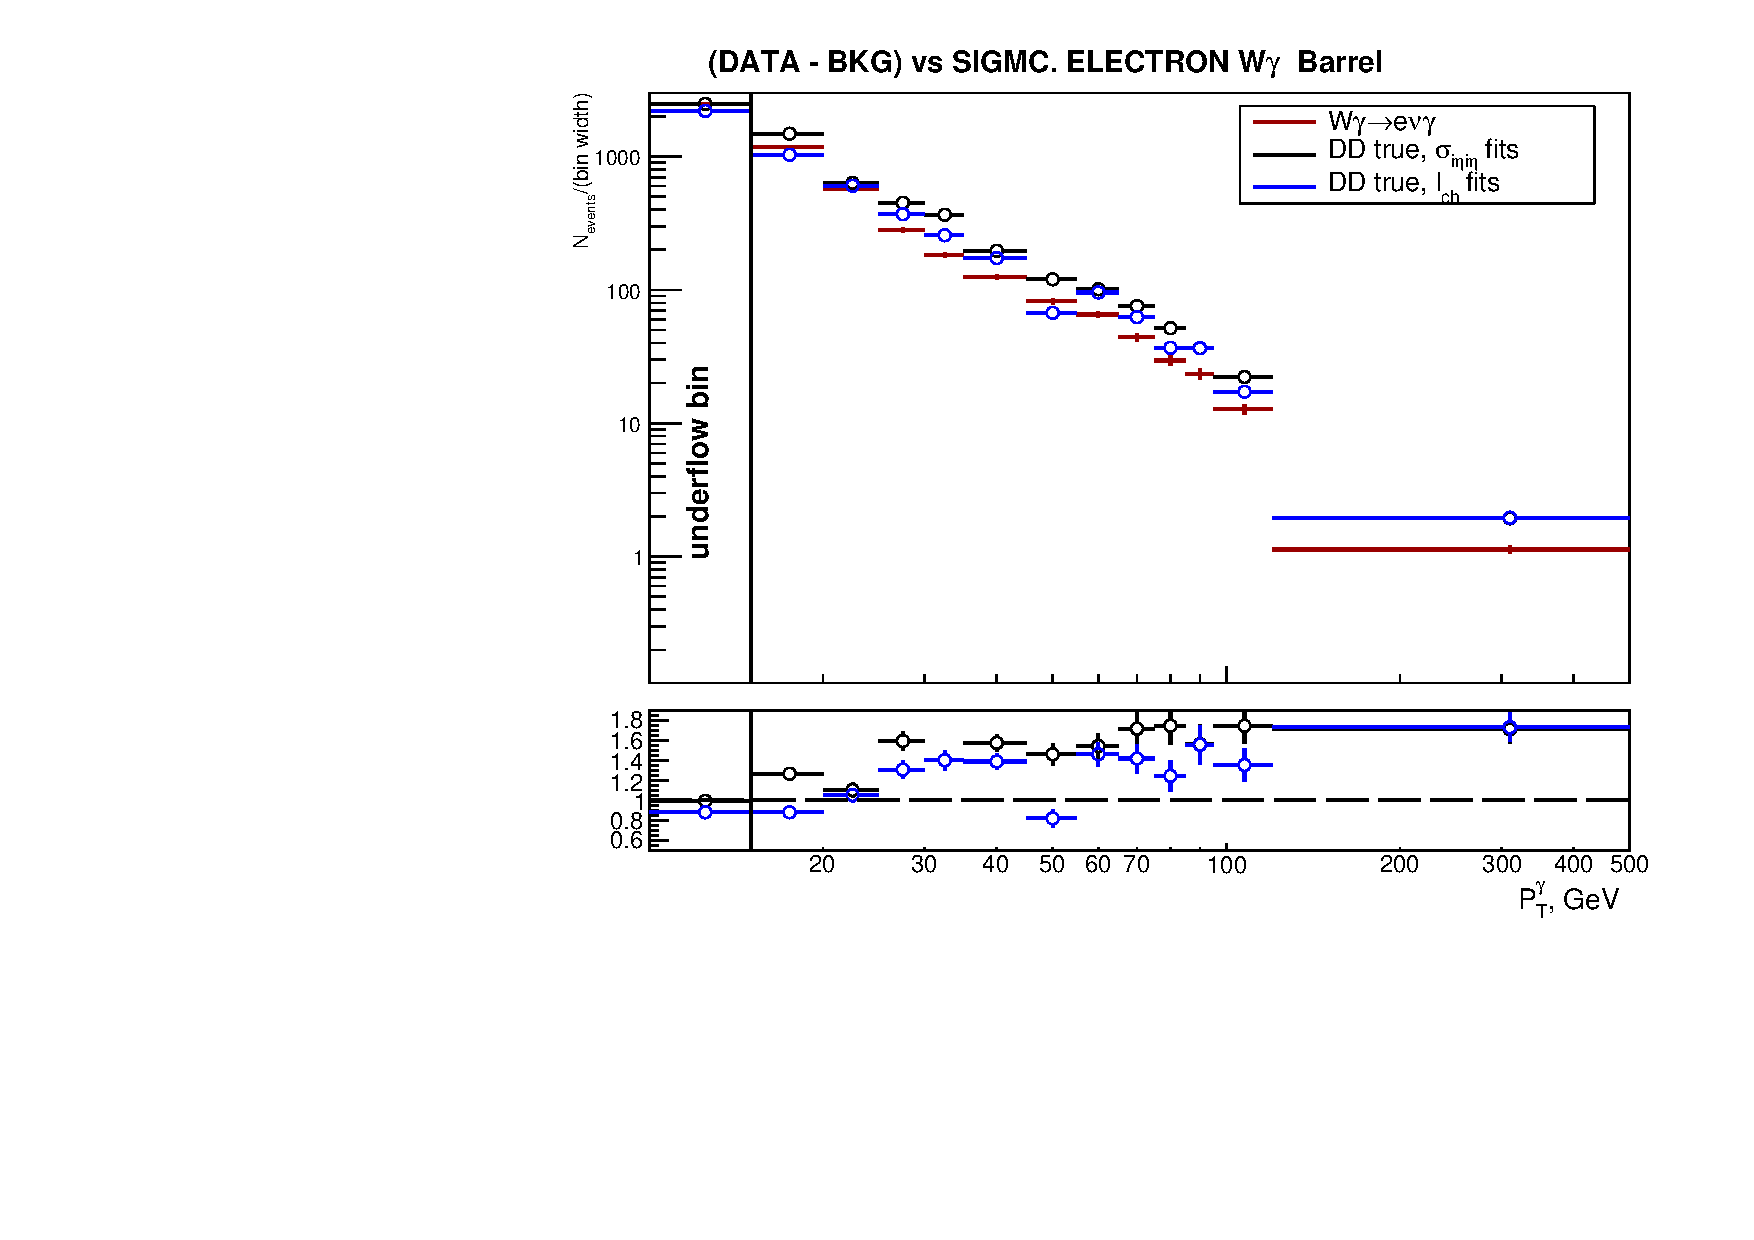
\includegraphics[width=0.40\textwidth]{../figs/figs_v11/ELECTRON_WGamma/PrepareYields/c_BkgSubtrDATAvsSIGMC_c_ELECTRON_WGamma__UNblind__Barrel__phoEt.pdf}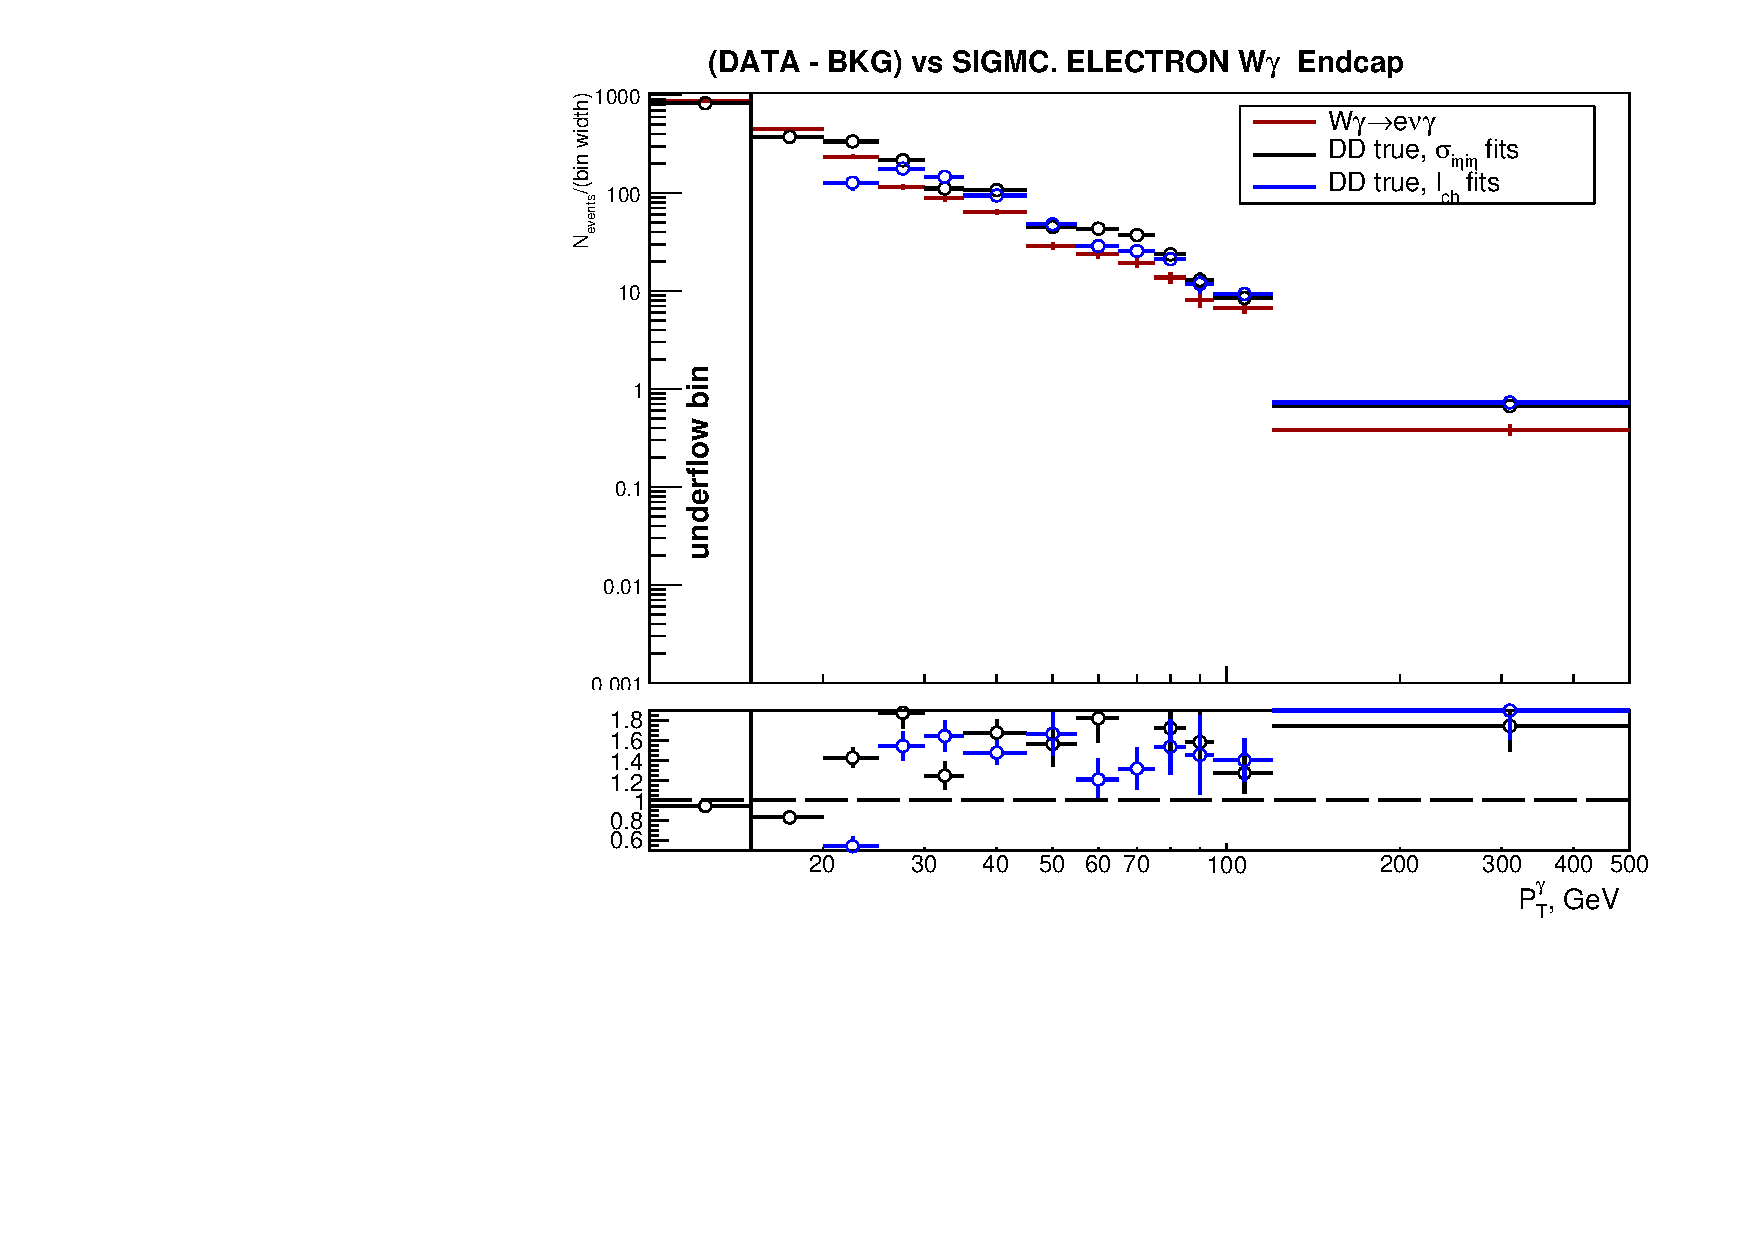
\includegraphics[width=0.40\textwidth]{../figs/figs_v11/ELECTRON_WGamma/PrepareYields/c_BkgSubtrDATAvsSIGMC_c_ELECTRON_WGamma__UNblind__Endcap__phoEt.pdf}\\
    \end{center}
  \end{figure}
\end{frame}%{$jets \rightarrow \gamma$ Background Subtraction. Plots, W$\gamma$}

\begin{frame}\frametitle {Cross Checks for Jets$\rightarrow\gamma$ Background Estimation}

\footnotesize{\bfseries{Simple MC closure check:}}
\tiny
\begin{itemize}
  \item Mix $W\gamma$ and $W$+jets MC samples to prepare pseudodata;
  \item Use $W\gamma$ and $W$+jets Mc to prepare templates;
  \item Fit pseudodata and compare fit results with MC predictions;
  \item Agreement is mostly good.
\end{itemize}

\footnotesize{\bfseries{MC realistic check:}}
\tiny
\begin{itemize}
  \item Mix $W\gamma$, $W$+jets, DY+jets, $Z\gamma$, $t\bar{t}$+jets MC samples to prepare pseudodata-I;
  \item Mix $Z\gamma$ and DY+jets MC to prepare pseudodata-II for templates;
  \item Fit pseudodata-I and compare fit results with MC predictions;
  \item Agreement is better than in data but generally not very good.
\end{itemize}

\footnotesize{\bfseries{$Z\gamma$ check:}}
\tiny
\begin{itemize}
  \item Apply $Z\gamma$ selection on Double Muon and Double Electron datasets;
  \item Prepare templates the same way as for the $W\gamma$ measurement;
  \item Fit $Z\gamma$-selected datasets and compare fit results with MC predictions and $I_{ch}^{\gamma}$ vs $\sigma_{i\etai\eta}^{\gamma}$;
  \item Measure $Z\gamma$ cross section and compare to the published CMS~8~TeV result;
  \item Agreement is very good.
\end{itemize}

\footnotesize{\bfseries{Conclusions: }}\scriptsize{reasons of discrepancies in the $W\gamma$ measurement:  }
\scriptsize
\begin{itemize}
  \item Not accurate shape of templates; 
  \item Effect of a bis on the fit machinery.
\end{itemize}

\end{frame}%{Real-$\gamma$ Backgrounds}
